% \textbf{Title: Sampling 3}

Consider these signals.

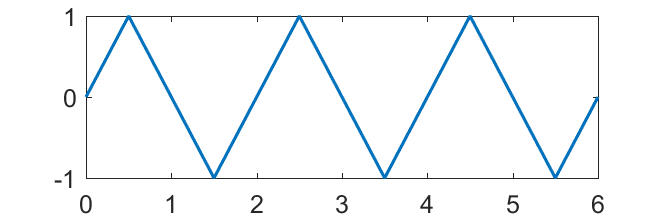
\includegraphics[width=3.05818in,height=1.01323in]{../../Images/SamplingAndAliasingQ3I.png}
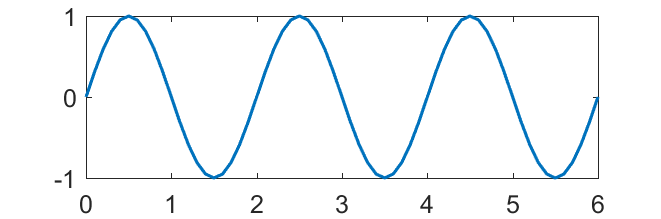
\includegraphics[width=3.06183in,height=1.01444in]{../../Images/SamplingAndAliasingQ3II.png}

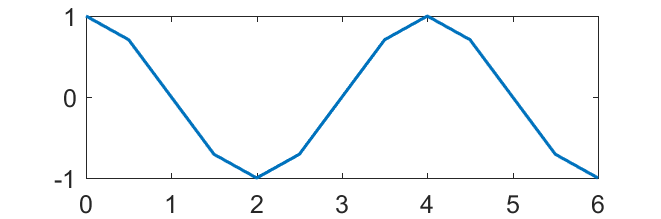
\includegraphics[width=3.08072in,height=1.02069in]{../../Images/SamplingAndAliasingQ3III.png}
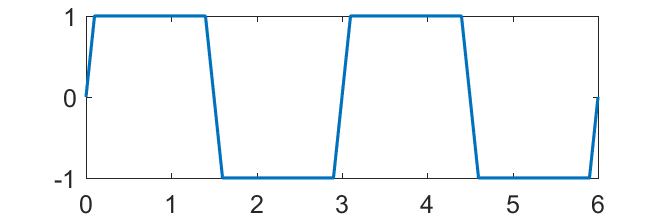
\includegraphics[width=3.08538in,height=1.02224in]{../../Images/SamplingAndAliasingQ3IV.png}

Which sampling period could cause all the reconstructed signals to become zero for some starting time? \\

*a. \(T_{s} = 6\) time units.

%@ Correct! This question tests the concept ``Sampling and Aliasing'', which is taught in these courses.

b. \(T_{s} = \frac{1}{6}\) time units.

%@ Incorrect. This question tests the concept ``Sampling and Aliasing'', which is taught in these courses.

c. \(T_{s} = 3\) time units.

%@ Incorrect. This question tests the concept ``Sampling and Aliasing'', which is taught in these courses.

d. \(T_{s} = 1\) time unit.

%@ Incorrect. This question tests the concept ``Sampling and Aliasing'', which is taught in these courses.

e. I do not know. \\

%@ It's okay. This question tests the concept ``Sampling and Aliasing'', which is taught in these courses.
